\documentclass{article}
\usepackage[paper=a4paper,margin=1in]{geometry}

\usepackage{listings}
\usepackage{graphicx}

\usepackage{amsmath}
%\usepackage{easyReview}

\newcommand{\titlelogoimage}{
\begin{figure}[h!]
    \centering
    
\includegraphics[width=1in]{images/logo.eps}
\end{figure}}

%opening
\title{Jib Instruction Set Architecture}
\author{Ian O'Rourke}
\date{\today \\ \titlelogoimage}

\lstset{basicstyle=\tiny,frame=single,captionpos=b}

\begin{document}

\maketitle

\section{Overview}

The Jib processor is a general-purpose Instruction Set Architecture (ISA). Each processor instruction is designed to take up exactly one word of memory. For Jib, each word takes up 32 bits; however, memory is addressable at the byte level. In cases where signed arithmetic is performed, signed integers are encoded using the two's-complement format. Jib also supports 32-bit floating point numeric algebra.

\subsection{Registers}

There are 32 total registers present on the Jib. These are defined generally as follows in Table \ref{table:register-setup}. Note that, as Jib is a 32-bit architecture, this means that each register is 32 bits wide. While there are specifications between general-purpose and system-level registers, any register is addressable and usable via standard instructions equally.

\begin{table}[h!]
    \centering
    \begin{tabular}{c|c}
        \hline
        Register & Usage \\
        \hline
        R0 & Program Counter \\
        R1 & Processor Status Flags \\
        R2 & Stack Pointer \\
        R3 & Excess / Overflow \\
        R4 & Return Register \\
        R5 & Argument Base Register \\
        R6-R31 & General Purpose Register \\
        \hline
    \end{tabular}
    \caption{Registers R0 through R5 are reserved for system-level parameters. All remaining registers are general-purpose.}
    \label{table:register-setup}
\end{table}

The program counter indicates the next instruction to be read. At the beginning of the processor cycle, the instruction at the memory address of the program counter is read in and processed. Then, the program counter is incremented at the end of each instruction cycle. If this value is needed to be modified, it is recommended to use the absolute \texttt{jmp}, or the relative jump instruction \texttt{jmpr} (see Section \ref{sec:instructions}), as opposed to writing to the register directly. This will automatically account for the increment at the end of the instruction cycle.

The global stack pointer maintains the global stack, as defined in Section \ref{sec:the-stack}. This provides the absolute address of the current stack location. Thus, when the stack is empty, it points to the stack base address, and when the stack is completely full it points to the memory location just above the last stack entry, or the base address plus the stack size. This value should not be edited by-hand to maintain the consistency of the program execution, but is instead modified by the stack instructions \texttt{push}, \texttt{pop}, \texttt{popr}, \texttt{call}, \texttt{ret}, \texttt{retint}, and \texttt{int}, as well as hardware interrupts. This should be loaded by the init program by assembly, however, to provide the default base location for the stack.

The return value instruction is intended to store the result of a function call, made using the \texttt{call} instruction. When the processor status flags are replaced with the caller's flags after the \texttt{ret} instruction is called, the return value is the only register that remains unchanged.

The processor status flags indicate the current setup for the processor. Currently, the following flags are assigned, as noted in Table \ref{table:processor-flags}.

\begin{table}[h!]
    \centering
    \begin{tabular}{l|l}
        \hline
        Bit & Value \\
        \hline
        0 & Interrupt Enable \\
        \hline
    \end{tabular}
    \caption{Processor status flags provide a window into the current processor state}
    \label{table:processor-flags}
\end{table}

This provides both a means to set and to read the current processor state values to ensure that the proper operating mode is configured for the currently-running program. This is maintained and replaced when \texttt{ret} and \texttt{retint} are called, so within an interrupt or function call, it is not necessary to replace the processor flags with those of the caller.

\subsection{Overall Instruction Syntax}

Since the architecture of the Jib is 32-bit, this means that the basic word, and therefore instruction format, exists in a 32-bit format. Note that, however, memory addresses are with respect to byte boundaries. Words are stored in big-endian format, meaning the most-significant component of the word is associated with the first byte in the word, while the least-significant component of the word is associated with the last byte in the word. Instructions must be placed with a base at a memory location with a byte alignment of four (e.g. 0, 4, 8, 12, etc.). General data may be placed and accessed from any byte alignment. The general instruction format is listed  in Table \ref{table:instruction-formatting}. The first byte, Byte 0, is always split into two components - the ID, composing the first 4 bits of the instruction, and the SubID, composing the next 4 bits of the instruction.

\begin{table}[h!]
    \centering
    \begin{tabular}{l|cccc}
        \hline
        {} & Byte 0 & Byte 1 & Byte 2 & Byte 3 \\
        Location & 0xFF000000 & 0x00FF0000 & 0x0000FF00 & 0x000000FF \\
        \hline
        Usage & opcode & arg0 & arg1 & arg2 \\
        Details & ID (\texttt{0xF0}), SubID (\texttt{0x0F}) & - & - & - \\
        \hline
    \end{tabular}
    \caption{The Jib instruction format typically has one opcode and three possible arguments associated with a particular opcode}
    \label{table:instruction-formatting}
\end{table}

This is contrasted with the typical assembly language formatting, which is provided as

\begin{center}
    \texttt{instruction <arg2> <arg1> <arg0>}
\end{center}

where the number of arguments depends on the required number of arguments for the instruction.

Certain arguments require type information. When this is present, the type code resides in the upper 3 bits of the argument byte (\texttt{0xE0}), while the register resides in the lower 5 bits (\texttt{0x1F}). Type codes are provided in Table \ref{table:type-codes}.

\begin{table}[h!]
	\centering
	\begin{tabular}{c|cc|c}
		\hline
		Type & Code & Size in Bytes & Description \\
		\hline
		 U8 & 1 & 1 & Unsigned byte \\
		 I8 & 2 & 1 & Signed byte \\
		 U16 & 3 & 2 & Unsigned short\\
		 I16 & 4 & 2 & Signed short \\
		 U32 & 5 & 4 & Unsigned integer \\
		 I32 & 6 & 4 & Signed integer \\
		 F32 & 7 & 4 & 32-bit floating point \\
		\hline
	\end{tabular}
	\caption{The supported type codes that are associated with certain instruction codes}
	\label{table:type-codes}
\end{table}

\subsection{Resetting}

On a hard-reset, all registers will be reset to 0 and memory values will be reset to their default values. The data parameter in memory at the hard-reset vector, stored at memory location 0, will be used as the reset vector.

On soft-reset, as called by the reset the program counter will be assigned the value contained in the soft-reset vector, which is stored at memory location 1. All of the other registers are reset to their default value of 0. Processor memory will be left unchanged and processor execution is then started.

On any reset, interrupts will be allowed by default.

\subsection{The Stack}
\label{sec:the-stack}

The stack pointer provides the absolute address of the stack pointer. The pointer points to the memory location just above the current stack location. If the stack is empty, the stack pointer points to the base address. Note that the base address is user-selectable, and there are no protections for stack under or overflow conditions, outside of wrapping around the minimum or maximum memory address, where the processor will error and halt.

\subsection{Interrupts}

Interrupts provide a means to interrupt the current flow of execution and run a separate method. There are two types of interrupts - hardware interrupts, which originate by request of an external hardware device, and software interrupts, which originate from a specific instruction. When an interrupt is triggered, the flow of program execution is interrupted before the next instruction is started. The current register state is stored on the stack, and the program counter is replaced with the value in the corresponding interrupt vector. Then, the program execution continues from this new location.

At the conclusion of any interrupt, the \texttt{retint} instruction should be called. This will replace the current register state with the values provided off the stack and resume program execution from the location right after the interrupt was called.

It should be noted that, if any values were pushed onto the stack during the interrupt handler, they should be popped off the stack prior to the \texttt{retint} call to avoid corrupting the program state.

The Jib supports 32 software and 32 hardware interrupts, as shown in Table \ref{table:interrupt-vector-locations}. The hardware interrupt vectors are stored in memory at locations \texttt{0x100} for interrupt 0 though \texttt{0x180}, exclusive, for interrupt 31. Similarly, the software interrupts are stored in memory at memory addresses \texttt{0x180} for interrupt 0 through \texttt{0x200}, exclusive, for interrupt 31.

\begin{table}[h!]
    \centering
    \begin{tabular}{c|ccccccc}
        \hline
        Type & 0 & 1 & 2 & \dots & 29 & 30 & 31 \\
        \hline
        Hardware & \texttt{0x100} & \texttt{0x104} & \texttt{0x108} & \dots & \texttt{0x174} & \texttt{0x178} & \texttt{0x17C} \\
        Software & \texttt{0x180} & \texttt{0x184} & \texttt{0x188} & \dots & \texttt{0x1F4} & \texttt{0x1F8} & \texttt{0x1FC} \\
        \hline
    \end{tabular}
    \caption{Interrupt vector locations for both hardware and software interrupts}
    \label{table:interrupt-vector-locations}
\end{table}

Note that, if a vector has a value of zero, that interrupt vector is considered to be disabled and that interrupt will effectively be disabled and not able to be run.

If an interrupt is not able to run immediately, due to interrupts being disabled, an interrupt request is placed into a single buffer. Once interrupts are re-enabled, if this queue is not empty, then that interrupt will be run. As this queue only has a size of one, if two interrupts are triggered at the same time, only the first interrupt will run. Any interrupt triggered while the queue is full will be silently discarded.

\pagebreak

\section{Instructions and Assembly Code}
\label{sec:instructions}

All available instructions are listed in Table \ref{table:instruction-table}. Note that any invalid instruction that is not provided in the table below results in an immediate halt of the processor. Note that, in the below logic, any indication where PC is incremented indicates that the standard \texttt{PC += 1} to move to the next instruction will be replaced by the logic provided in the description field. Note that, based on the type, for addresses, this can affect either just the memory location assigned by the register (for a single-byte type), the register byte and the following byte (for a two-byte type), or the register byte and the following three bytes (for a four-byte type). The user must ensure that the appropriate locations are valid and able to be written to when setting up the registers and types for particular instructions. Instruction formats, as denoted in the ``Format ID'' column, are located in Table \ref{table:instruction-format-types}.

\begin{table}[h!]
	\centering
	\begin{footnotesize}
		\begin{tabular}{c|cc|l|l}
			\hline
			Format ID & \multicolumn{2}{c|}{Opcode} & Assembly & Description \\
			{} & ID & SubID & {} & {} \\
			\hline
			A & 0 & 0 & \texttt{noop} & No Operation \\
			A & 0 & 1 & \texttt{reset} & \texttt{PC = Reset Vector}, \texttt{R[0-15] = 0} \\
			B & 0 & 2 & \texttt{int <imm>} & Trigger software interrupt number \texttt{imm} \\
			C & 0 & 3 & \texttt{intr [a]} & Trigger software interrupt number \texttt{R[a]} \\
			A & 0 & 4 & \texttt{retint} & $\forall_{i \in [31 \rightarrow 0]}$ \texttt{R[i] = mem[--SP]}, \texttt{++PC} \\
			C & 0 & 5 & \texttt{call [a]} &  $\forall_{i \in [0 \rightarrow 31]}$ \texttt{mem[SP++] = R[i]}; \texttt{PC = R[a]} \\
			A & 0 & 6 & \texttt{ret} & $\forall_{i \in [31 \rightarrow 0], i \not= \$ret}$ \texttt{R[i] = mem[--SP]}, \texttt{++PC} \\
			C & 0 & 7 & \texttt{push [a]} & \texttt{mem[SP += 4] = R[a]} \\
			A & 0 & 8 & \texttt{pop} & \texttt{SP -= 4} \\
			C & 0 & 9 & \texttt{popr [a]} & \texttt{R[a] = mem[SP -= 4]} \\
			C & 0 & 10 & \texttt{jmp [a]} & \texttt{PC = R[a]} \\
			C & 0 & 11 & \texttt{jmpr [a]} & \texttt{PC += R[a]} \\
			B & 0 & 12 & \texttt{jmpri <imm>} & \texttt{PC += Imm} (Signed) \\
			A & 0 & 15 & \texttt{halt} & Stop Program Execution \\

			G & 1 & 0 & \texttt{ld [a] [b]} & \texttt{R[a] = mem[R[b]]} \\
			G & 1 & 1 & \texttt{ldr [a] [b]} & \texttt{R[a] = mem[PC + R[b]]} \\
			E & 1 & 2 & \texttt{ldi [dst] <imm>} & \texttt{R[dst] = Im} \\
			E & 1 & 3 & \texttt{ldri [dst] <imm>} & \texttt{R[dst] = mem[PC + Im]} \\
			D & 1 & 4 & \texttt{ldn [a]} & \texttt{R[a] = mem[PC + 1]}, \texttt{PC += 2} \\
			G & 1 & 5 & \texttt{sav [a] [b]} & \texttt{mem[R[a]] = R[b]} \\
			G & 1 & 6 & \texttt{savr [a] [b]} & \texttt{mem[PC + R[a]] = R[b]} \\
			F & 1 & 7 & \texttt{copy [a] [b]} & \texttt{R[a] = R[b]} \\
			H & 1 & 8 & \texttt{conv [a] [b]} & \texttt{R[a] = R[b]} \\

			I & 2 & 0 & \texttt{teq [dst] [a] [b]} & If \texttt{R[a] == R[b]} \texttt{R[dst] = 1}, Else \texttt{R[dst] = 0} \\
			I & 2 & 1 & \texttt{tneq [dst] [a] [b]} & If \texttt{R[a] != R[b]} \texttt{R[dst] = 1}, Else \texttt{R[dst] = 0} \\
			I & 2 & 2 & \texttt{tg [dst] [a] [b]} & If \texttt{R[a] > R[b]} \texttt{R[dst] = 1}, Else \texttt{R[dst] = 0} \\
			I & 2 & 3 & \texttt{tge [dst] [a] [b]} & If \texttt{R[a] >= R[b]} \texttt{R[dst] = 1}, Else \texttt{R[dst] = 0} \\
			I & 2 & 4 & \texttt{tl [dst] [a] [b]} & If \texttt{R[a] < R[b]} \texttt{R[dst] = 1}, Else \texttt{R[dst] = 0} \\
			I & 2 & 5 & \texttt{tle [dst] [a] [b]} & If \texttt{R[a] <= R[b]} \texttt{R[dst] = 1}, Else \texttt{R[dst] = 0} \\

			F & 3 & 0 & \texttt{not [dst] [a]} & If \texttt{R[a] != 0} \texttt{R[dst] = 0}, Else \texttt{R[dst] = 1} \\
			F & 3 & 1 & \texttt{bool [dst] [a]} & If \texttt{R[a] != 0} \texttt{R[dst] = 1}, Else \texttt{R[dst] = 0} \\
			C & 3 & 2 & \texttt{tz [a]} & If \texttt{R[a] == 0} \texttt{PC += 1}, Else \texttt{PC += 2} \\
			C & 3 & 3 & \texttt{tnz [a]} & If \texttt{R[a] != 0} \texttt{PC += 1}, Else \texttt{PC += 2} \\

			A & 4 & 0 & \texttt{inton} & Turn Interrupts On \\
			A & 4 & 1 & \texttt{intoff} & Turn Interrupts Off \\

            A & 5 & 0 & \texttt{brk} & Debug Breakpoint (capturable by hardware; otherwise, acts as a \texttt{noop}) \\

			I & 10 & 0 & \texttt{add [dst] [a] [b]} & \texttt{R[dst] = R[a] + R[b]} \\
			I & 10 & 1 & \texttt{sub [dst] [a] [b]} & \texttt{R[dst] = R[a] - R[b]} \\
			I & 10 & 2 & \texttt{mul [dst] [a] [b]} & \texttt{R[dst] = R[a] * R[b]} \\
			I & 10 & 3 & \texttt{div [dst] [a] [b]} & \texttt{R[dst] = R[a] / R[b]} \\
			I & 10 & 4 & \texttt{rem [dst] [a] [b]} & \texttt{R[dst] = R[a] \% R[b]} \\
			G & 10 & 5 & \texttt{neg [dst] [a]} & \texttt{R[dst] = -R[a]} \\

			I & 11 & 0 & \texttt{band [dst] [a] [b]} & \texttt{R[dst] = R[a] \& R[b]} \\
			I & 11 & 1 & \texttt{bor [dst] [a] [b]} & \texttt{R[dst] = R[a] | R[b]} \\
			I & 11 & 2 & \texttt{bxor [dst] [a] [b]} & \texttt{R[dst] = R[a] $\wedge$ R[b]} \\
			I & 11 & 3 & \texttt{bshl [dst] [a] [b]} & \texttt{R[dst] = R[a] << R[b]} \\
			I & 11 & 4 & \texttt{bshr [dst] [a] [b]} & \texttt{R[dst] = R[a] >> R[b]} \\
			G & 11 & 5 & \texttt{bnot [dst] [a]} & \texttt{R[dst] = \textasciitilde R[a]} \\
			\hline
		\end{tabular}
	\end{footnotesize}
	\caption{Available instruction list for the Jib provides a variety of commands.}
	\label{table:instruction-table}
\end{table}

There are several different types of instruction formats, which make use of the four byte spots in the instruction opcode slightly differently. These are provided below in Table \ref{table:instruction-format-types}. As the first byte, Byte 0, is always the same, it is omitted from the table below. See Table \ref{table:instruction-formatting} for more details on Byte 0. Most commonly, and instruction will only use a single type for all registers present in the operation. Some instructions, in particular conversion instructions, will use multiple type codes for different registers.

\begin{table}[h!]
	\centering
	\begin{tabular}{cc|ccc}
		\hline
		ID & Name & Byte 1 & Byte 2 & Byte 3 \\
		\hline
		A & No Argument & - & - & - \\
		B & Immediate (i16) & - & Imm (\texttt{0xF0}) & Imm (\texttt{0x0F}) \\
		C & Single Register & Register & - & - \\
		D & Single Register Type & Register Type & - & - \\
		E & Single Register Immediate & Register Type & Imm (\texttt{0xF0}) & Imm (\texttt{0x0F}) \\
		F & Double Register & Register & Register & - \\
		G & Double Register Type & Register Type & Register & - \\
		H & Conversion & Register Type & Register Type & - \\
		I & Arithmetic & Register Type & Register & Register \\
		\hline
	\end{tabular}
	\caption{Instructions can take a variety of different forms depending on the needs of the operation}
	\label{table:instruction-format-types}
\end{table}

\pagebreak

The assembler also has several commands available, detailed in Table \ref{table:assembler-commands}. Note that, for the \texttt{.loadtext} command, the text will be loaded in via the character map provided in Section \ref{sec:character-map}.

\begin{table}[h!]
    \centering
    \begin{tabular}{l|l}
        \hline
        Command & Description \\
        \hline
        \texttt{:[label]} & Defines a new label associated with the current memory location \\
        \texttt{.oper [offset]} & Changes the current assembly offset to the value provided \\
        \texttt{.load [num]} & Loads the data value as either an unsigned word (if in hex or positive)\\
        & or as a signed word (if negative) in the current memory location \\
        \texttt{.loadloc [label]} & Loads the data index associated with the provided label into \\
        & the current memory location \\
        \texttt{.loadtext "[TEXT]"} & Loads the text into memory, starting at the current memory location, \\
        & placing each character into the next subsequent memory location, with \\
        & a null-terminator as copied into memory after the text value \\
        \hline
    \end{tabular}
    \caption{Available assembler commands}
    \label{table:assembler-commands}
\end{table}

Reference names are available to link to the special register values, as listed in Table \ref{table:assembler-register-references}.

\begin{table}[h!]
    \centering
    \begin{tabular}{l|cl}
        \hline
        Reference Name & Register & Description \\
        \hline
        \texttt{\$pc} & 0 & Program Counter \\
        \texttt{\$stat} & 1 & Status Flags \\
        \texttt{\$sp} & 2 & Stack Pointer \\
        \texttt{\$ovf} & 3 & Overflow \\
        \texttt{\$ret} & 4 & Return \\
        \texttt{\$arg} & 5 & Argument Base \\
        \hline
    \end{tabular}
    \caption{Assembler provides shortcuts for commonly-referenced register indices}
    \label{table:assembler-register-references}
\end{table}

\subsection{Calling Convention}

The calling convention...

\pagebreak

\section{Character Mapping}
\label{sec:character-map}

Jib computers, by default, utilize the following character map. This is similar to the American Standard Code for Information Interchange (ASCII) format. The Jib character map is defined in Table \ref{table:character-map}. Any undefined entries in the character map are considered invalid characters.

\newcommand{\charmap}[1]{\texttt{#1}}

\newcommand{\charslash}{\texttt{\char`\\}}

\newcommand{\charmapescape}[1]{\charmap{\texttt{\charslash#1}}}

\begin{table}[h!]
    \centering
    \begin{tabular}{cc|cc|cc|cc}
        \hline
        Hex & Char & Hex & Char & Hex & Char & Hex & Char \\
        \hline
        00 & \charmapescape{0} NULL & 20 & Space & 40 & \charmap{@} & 60 & \charmap{`} \\
        01 & {} & 21 & \charmap{!} & 41 & \charmap{A} & 61 & \charmap{a} \\
        02 & {} & 22 & \charmap{"} & 42 & \charmap{B} & 62 & \charmap{b} \\
        03 & {} & 23 & \charmap{\#} & 43 & \charmap{C} & 63 & \charmap{c} \\
        04 & {} & 24 & \charmap{\$} & 44 & \charmap{D} & 64 & \charmap{d} \\
        05 & {} & 25 & \charmap{\%} & 45 & \charmap{E} & 65 & \charmap{e} \\
        06 & {} & 26 & \charmap{\&} & 46 & \charmap{F} & 66 & \charmap{f} \\
        07 & {} & 27 & \charmap{\textquotesingle} & 47 & \charmap{G} & 67 & \charmap{g} \\
        08 & {} & 28 & \charmap{(} & 48 & \charmap{H} & 68 & \charmap{h} \\
        09 & {} & 29 & \charmap{)} & 49 & \charmap{I} & 69 & \charmap{i} \\
        0A & \charmapescape{n} New Line & 2A & \charmap{*} & 4A & \charmap{J} & 6A & \charmap{j} \\
        0B & {} & 2B & \charmap{+} & 4B & \charmap{K} & 6B & \charmap{k} \\
        0C & {} & 2C & \charmap{,} & 4C & \charmap{L} & 6C & \charmap{l} \\
        0D & {} & 2D & \charmap{-} & 4D & \charmap{M} & 6D & \charmap{m} \\
        0E & {} & 2E & \charmap{.} & 4E & \charmap{N} & 6E & \charmap{n} \\
        0F & {} & 2F & \charmap{/} & 4F & \charmap{O} & 6F & \charmap{o} \\
        10 & {} & 30 & \charmap{0} & 50 & \charmap{P} & 70 & \charmap{p} \\
        11 & {} & 31 & \charmap{1} & 51 & \charmap{Q} & 71 & \charmap{q} \\
        12 & {} & 32 & \charmap{2} & 52 & \charmap{R} & 72 & \charmap{r} \\
        13 & {} & 33 & \charmap{3} & 53 & \charmap{S} & 73 & \charmap{s} \\
        14 & {} & 34 & \charmap{4} & 54 & \charmap{T} & 74 & \charmap{t} \\
        15 & {} & 35 & \charmap{5} & 55 & \charmap{U} & 75 & \charmap{u} \\
        16 & {} & 36 & \charmap{6} & 56 & \charmap{V} & 76 & \charmap{v} \\
        17 & {} & 37 & \charmap{7} & 57 & \charmap{W} & 77 & \charmap{w} \\
        18 & {} & 38 & \charmap{8} & 58 & \charmap{X} & 78 & \charmap{x} \\
        19 & {} & 39 & \charmap{9} & 59 & \charmap{Y} & 79 & \charmap{y} \\
        1A & {} & 3A & \charmap{:} & 5A & \charmap{Z} & 7A & \charmap{z} \\
        1B & {} & 3B & \charmap{;} & 5B & \charmap{[} & 7B & \charmap{\{} \\
        1C & {} & 3C & \charmap{<} & 5C & \charmap{\charslash} & 7C & \charmap{|} \\
        1D & {} & 3D & \charmap{=} & 5D & \charmap{]} & 7D & \charmap{\}} \\
        1E & {} & 3E & \charmap{>} & 5E & \charmap{\textasciicircum} & 7E & \charmap{\textasciitilde} \\
        1F & {} & 3F & \charmap{?} & 5F & \charmap{\textunderscore} & 7F & {} \\
        \hline
    \end{tabular}
    \caption{Jib character mapping}
    \label{table:character-map}
\end{table}

\pagebreak

\section{Devices}
\label{sec:devices}

Devices are memory-mapped in Jib. This means that reading or writing to special regions in memory facilitate the communication with these external devices. In a typical Jib computer, the device region consists of up to 64 devices, starting at memory address \texttt{0xA000}, with each device allocating up to 32 bytes of memory. Not all devices will make use all the available memory slots for a given device. In these cases, a memory exception will be provided if any of these invalid addresses are read from or written to.

\subsection{Serial Input and Output}

The serial input and output device is one of the simplest devices. It essentially consists of a device two queues, one for input, and another for output. Each of these queues has an internal buffer size of 256 words. If any words are attempted to be added to the queue once either queue is full, no additional data is read and that data is lost.

The memory mapping for the serial input and output device is provided in Table \ref{table:dev-serial-io}.

\begin{table}[h!]
    \centering
    \begin{tabular}{l|lll}
        \hline
        Offset & Type & Read/Write & Usage \\
        \hline
        \texttt{0} & u16 & Read & Device ID 1 \\
        \texttt{2} & u8 & Read & Provides the current input queue size \\
        \texttt{3} & u8 & Read & Pops and provides a word off the front of the input queue \\
        & & & If no data is available, will return \texttt{0} by default \\
        \texttt{4} & u8 & Read & Provides the current output queue size \\
        \texttt{5} & u8 & Write & Pushes a word onto the output queue \\
        \texttt{6} & u8 & Write & Clears the input queue if the value written is nonzero \\
        \texttt{7} & u8 & Write & Clears the output queue if the value written is nonzero \\
        \hline
    \end{tabular}
    \caption{Serial Input and Output device provides a simple data structure to read and write data streams}
    \label{table:dev-serial-io}
\end{table}

\subsection{IRQ Clock}

The IRQ clock provides a means to trigger a specific hardware interrupt at a regular interval of clock cycles. This consists of a settable interval (or set to 0 to disable), as well as a settable interrupt to trigger. Available in memory is the ability to read any of these two settable parameters, as well as a readable indication of the current clock cycle count. The memory mapping is provided in Table \ref{table:dev-irq-clock}.

\begin{table}[h!]
	\centering
	\begin{tabular}{l|lll}
		\hline
		Offset & Type & Read/Write & Usage \\
		\hline
		\texttt{0} & u16 & Read & Device ID 2 \\
		\texttt{2} & u32 & Read/Write & Gets/sets the clock interval in CPU cycles. Set to 0 to disable. \\
		\texttt{6} & u32 & Read & Provides the current clock counter in CPU cycles. \\
		{} & {} & {} & Will be between 0 and the above interval. \\
		\texttt{10} & u32 & Read/Write & The hardware IRQ to trigger. \\
		\hline
	\end{tabular}
	\caption{Serial Input and Output device provides a simple data structure to read and write data streams}
	\label{table:dev-irq-clock}
\end{table}

\pagebreak

\section{Examples}

The following list some simple example programs that can be run on the Jib.

\subsection{Counter}

The program listed in Listing \ref{listing:example-counter} provides a basic counter. A target value is placed in register four, and the value in register three is incremented from 0 to the target value in register four by adding one to the register each loop. Once the target value has been reached and register three is equal to register four, the program halts by entering an infinite loop.

\lstinputlisting[caption={Limited counter program}, label={listing:example-counter}]{../jib-asm/examples/counter.jsm}

\pagebreak
\subsection{Infinite Counter}

Listing \ref{listing:example-infinite-counter} makes use of some additional functionality, including the use of the register reference names, to test register reset functionality. It also modifies the program counter outside of the standard jump command.

\lstinputlisting[caption={Infinite counter program with register reference names}, label={listing:example-infinite-counter}]{../jib-asm/examples/infinite_counter.jsm}

\subsection{Hello World}

Listing  \ref{listing:hello-world} provides a program that will infinitely write "hello, world" to the serial device, expected to be memory-mapped into the Jib at \texttt{0xA000}. This makes use of the \texttt{.loadtext} command, which loads the text, and an additional null-terminator at the end, directly into memory. It also makes use of a print-string function call to handle printing string values to the serial output devices.

\lstinputlisting[caption={Infinite "hello, world!" program}, label={listing:hello-world}]{../jib-asm/examples/hello_world.jsm}

\pagebreak

\subsection{Serial Echo}

Listing \ref{listing:serial-echo} provides a serial echo program, which echos any text provided by the default serial input device back out via the serial echo device. This serial device is expected to be provided at the starting location \texttt{0xA000}.

\lstinputlisting[caption={Serial echo program reads in text characters and immediately outputs via the output device}, label={listing:serial-echo}]{../jib-asm/examples/serial_echo.jsm}

\pagebreak

\section{C/Buoy}

C/Buoy is a higher-level language than the raw assembly that provides some nicer tools to program applications in, at the cost of being less space and time efficient than programming in assembly directly. It does offer a slightly safer method of computing, however, as it provides a more traditional function call structure, variables, and scopes that help abstract away some of the hardware and provide some simple limits on what the user is allowed to do.

Note that, in this case, both functions and variables share the same namespace. This allows for easy use of function pointers by variable names, though currently only names are allowed, and no expressions may be used as yet.

\begin{table}[h!]
\begin{tabular}{rl}
    Program & $\rightarrow$ \\
    & \textlangle BaseStatement\textrangle \\
    BaseStatement & $\rightarrow$ \\
    & \textlangle BaseStatement\textrangle \textlangle BaseStatement\textrangle \\
    & fn \texttt{FunctionName}(\texttt{Variable}[, \texttt{Variable}\dots]) \{ \textlangle StatementList\textrangle \} \\
    & static VarType \texttt{Variable}[ = \textlangle BaseExpression\textrangle]; \\
    Statement & $\rightarrow$ \\
    & def \texttt{Variable}: \textlangle VarType\textrangle [ = \textlangle BaseExpression\textrangle]; \\
    & return; \\
    & return \textlangle BaseExpression\textrangle; \\
    & \textlangle BaseExpression\textrangle; \\
    & \{ \textlangle StatementList\textrangle \} \\
    & if (\textlangle BaseExpression\textrangle) \textlangle Statement\textrangle \\
    & if (\textlangle BaseExpression\textrangle) \textlangle Statement\textrangle else \textlangle Statement\textrangle \\
    & while (\textlangle BaseExpression\textrangle) \textlangle Statement\textrangle \\
    StatementList & $\rightarrow$ \\
    & \textlangle Statement\textrangle \\
    & \textlangle Statement\textrangle \textlangle Statement\textrangle \\
    BaseExpression & $\rightarrow$ \\
    & \textlangle Expression\textrangle = \textlangle BaseExpression\textrangle \\
    & \textlangle Expression\textrangle \textlangle BinaryOp\textrangle \textlangle Expression\textrangle \\
    & \textlangle Expression\textrangle \\
    Expression & $\rightarrow$ \\
    & \texttt{Variable} \\
    & \textlangle Literal\textrangle \\
    & \textlangle UnaryOp\textrangle \textlangle Expression\textrangle \\
    & \texttt{FunctionName}([\textlangle BaseExpression\textrangle[, \textlangle BaseExpression\textrangle,\dots]]) \\
    & (\textlangle BaseExpression\textrangle) \\
    BinaryOp & $\rightarrow$  \\
    & +, -, *, /, \textless, \textgreater, \textless=, \textgreater=, \&\&, \textbar\textbar, \&, \textbar, ==, !=\\
    UnaryOp & $\rightarrow$ \\
    & *, -, +, !, \textasciitilde \\
    VarType & $\rightarrow$ \\
    & auto \\
    & auto[\textlangle WordLiteral\textrangle] \\
    & [int, uint] \\
\end{tabular}
\end{table}

This makes use of a few extra conventions. At the start of each function, stack space is reserved both for any local variables, as well as any temporary variables, that are required. A few extra registers are defined in the Table \ref{table:cbuoy-register-references} below.

\begin{table}[h!]
    \centering
    \begin{tabular}{l|cl}
        \hline
        Register & Description \\
        \hline
        6 & Function Local Variables  \\
        7 & Function Temporary Variables \\
        8 & Spare Register \\
        \hline
    \end{tabular}
    \caption{Additional registers defined/allocated for use by C/Buoy}
    \label{table:cbuoy-register-references}
\end{table}

When returning a parameter, if the parameter is a primitive, it is returned by value in the return register directly. However, if it is a structure, the address of the temporary to write into is written into the return register before the function call. This is typically a temporary allocated on the stack, as mentioned above.

This provides an example program in Listing \ref{listing:example-cbuoy} below, which provides an example of printing text to a serial device, both using a string literal, but also converting numeric values into their text equivalents.

\lstinputlisting[label={listing:example-cbuoy},caption={Example C/Buoy program for printing out a string to a serial output device}]{../cbuoy/examples/printing.cb}

\pagebreak

\section{Tools}

Several tools can help in the development of Jib programs.

\subsection{V/Jib}

One useful tool is \texttt{V/Jib}, combines together a basic assembler, CPU emulator, and memory inspector into a single program. The main window can be seen in Figure \ref{fig:visual-jib-main-page}.

\begin{figure}[h!]
    \centering
    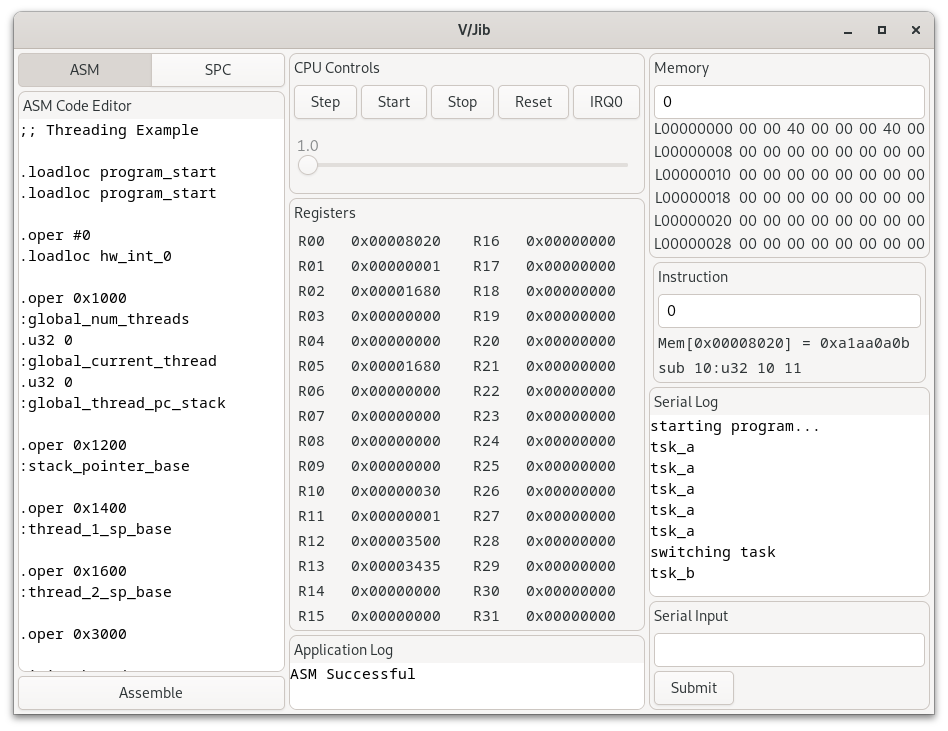
\includegraphics[width=5in]{images/visual-jib.png}
    \caption{Main window of \texttt{V/Jib} provides common tools for program writing}
    \label{fig:visual-jib-main-page}
\end{figure}


\end{document}
